\documentclass{article}
\usepackage{graphicx}
\begin{document}
Tameez Latib

Problem 6

I, Tameez Latib, declare that this work is my own. I did this work honestly and can fully stand behind everything that I have written.

---

First, let's consider hot water cooling down due to the environment. The experimental data from measuring the temperature of the water is as follows (With T(t) = Temperature after time t)

$T(0s) =  95.7^oC$

$T(50s) =  91.4^oC$

$T(100s) =  88.2^oC$

$T(150s) =  85.4^oC$

$T(200s) =  82.7^oC$

To model this, we will use Newton's law of cooling: 

$$\frac{dT}{dt} = k(T-T_a)$$

Where $T_a$ is the ambient temperature, and k is a constant depending on the substance. This can be simplified to:

$$T(t) = T_a + (T_0 - T_a)e^{-kt}$$

With $T_0$ being the initial temperature. 

In our case, we will assume $T_a$ is fixed at $21^oC$, and $T_0 = 95.7^oC$

Solving our equation in terms of k, we get

$$T = T_a + (T_0 - T_a)e^{-kt}$$

$$\frac{(T-T_a)}{(T_0 - T_a)} = e^{-kt}$$

$$ln(\frac{(T-T_a)}{(T_0 - T_a)}) = -kt$$

$$k = -ln(\frac{(T-T_a)}{(T_0 - T_a)})*\frac{1}{t}$$

Using this, and plugging in our values, k is determined for each (t, T) value pair.

$k = 0.00119/s$,
 
$k = 0.00105/s$,

$k = 0.00099/s$, 

$k = 0.00096/s$, 

So lets take the average of these values for our actual k value.

$$k = 0.00105/s$$

Let's see if our model is valid:

$T(t) = 21 + (74.7)e^{-0.00105t}$ (omitted units for simplicity)

$T(50s) = 91.9^oC$

$T(100s) = 88.3^oC$

$T(150s) = 84.8^oC$

$T(200s) = 81.6^oC$

Looking back at our data, the result is accurate, differing only by $1^oC$ at most. 



\vspace{2cm}

Now, let's consider a different experiment, a rod is placed into water with unknown Temperature, with the temperature of the rod given t various time intervals

$T(0s) =  92.0^oC$

$T(5s) =  38.6^oC$

$T(10s) =  28.4^oC$

$T(15s) =  24.8^oC$

$T(20s) =  23.3^oC$

Similarly, Newton's law of cooling gives us:

$$T = T_a + (T_0 - T_a)e^{-kt}$$

Where both k and $T_a$ are unknown, as $T_a$ is the temperature of the water. 

From the second and last data points (we use the last data point to avoid the data being inaccurate, as the start and end data points give us the greatest range- the greatest region (the whole range in this case) in which the model should be accurate.)

$$38.6 = T_a + (T_0 - T_a)e^{-k*5}$$

$$23.3 = T_a + (T_0 - T_a)e^{-k*20}$$

(Note: since we know the units match up, I will omit them for simplicity) This is just a system of equations with 2 unknowns and 2 equations. 
By algebra, the following two equations are found 

$$\frac{(38.6 -T_a)}{(T_0 - T_a)}=  (e^{-k})^5$$

$$\frac{(23.3 -T_a)}{(T_0 - T_a)}=  (e^{-k})^{20}$$

Raising the first of these equations to the 4th power, and then substituting it for the right hand side of the second, we attain

$$\frac{(23.3 -T_a)}{(T_0 - T_a)}=\frac{(38.6 -T_a)^4}{(T_0 - T_a)^4}$$

Where $T_0=92$, a numeric solver determines 

$T_a = 23.1^oC$

Plugging this in to:

$$k = -ln(\frac{(T-T_a)}{(T_0 - T_a)})*\frac{1}{t}$$

For all values of (t, T), We get 

$k = 0.298/s$

$k = 0.256/s$

$k = 0.247/s$

$k = 0.292/s$

Taking the average, $k = 0.273$

Let's try see if our model is valid for these values for k and $T_a$, we have

$T(t) = 23.1 + (68.9)e^{-0.273t}$ (units omitted for simplicity)

$T(5s) = 40.7^oC$

$T(10s) = 27.6^oC$

$T(15s) = 24.2^oC$

$T(20s) = 23.4^oC$

While the values are not perfect, they are pretty accurate- off by about $2^oC$ at most.

\vspace{2cm}

Lastly, let's look at the case of a rod at room temperature ($21^oC$) immersed into water at temperature $95^oC$
First, let's list known data

$T_a = 21^oC$

$T_w(0s) = 95^oC$

$T_r(0s) = 21^oC$ 

$k_w = 0.00105/s$

$k_r = 0.273/s$

In fact, we know 

$T_w(t) = 21+(95-21)e^{-0.00105t}$ (omitting units) 

$$T_w(t) = 21+(74)e^{-0.00105t}$$

From simply plugging in to our equation from experiment 1, with $T_0 = 95^oC$, as we can assume the rod's effect on the water is negligible as the water has a much larger volume than the rod, so the ambient air will be the only factor.

Furthermore, the ambient temperature for the rod would be the water, as that surrounds it. However, we must be careful as $T_a = T_w(t)$ is now a function of t. So going back to the differential equation from Newton's law of cooling:

$$\frac{dT_r(t)}{dt} = -k_r(T_r(t)-T_w(t))$$

$$\frac{dT_r(t)}{dt} = -k_r(T_r(t)-21-(74)e^{-0.00105t})$$

$$\frac{dT_r(t)}{dt} = -k_r(T_r(t)-21)+k_r(74)e^{-0.00105t})$$

Let $$x = T_r - 21$$. This substitution makes the equation slightly better, as $$\frac{dx}{dt} = \frac{dT_r(t)}{dt}$$

$$\frac{dx}{dt} = -k_r(x)+k_r(74)e^{-0.00105t})$$

$$\frac{dx}{dt}+k_rx =k_r(74)e^{-0.00105t})$$

Multiply by $u$, an unknown function where 

$ux' + uk_rx = (ux)' = ux' + u'x$

$u' = uk_r$

$u = e^{k_r*t}$

Now we have

$$\frac{d(xe^{k_r*t})}{dt} = 74e^{k_r*t}k_re^{-0.00105t}$$

$$xe^{k_r*t} = \int74k_re^{-0.00105t+k_rt}dt$$

$$xe^{k_r*t} = \frac{74k_re^{(-0.00105+k_r)t}}{(-0.00105+k_r)}+C$$

$$x = \frac{74k_re^{(-0.00105)t}}{(-0.00105+k_r)}+Ce^{-k_rt}$$

Finally, 

$$T_r(t) = 21 + \frac{74k_re^{(-0.00105)t}}{(-0.00105+k_r)}+Ce^{-k_rt}$$

With $k_r = 0.273$

$$T_r(t) = 21 + \frac{20.2e^{(-0.00105)t}}{0.272}+Ce^{-0.273t}$$

$$T_r(t) = 21 +74.23e^{(-0.00105)t}+Ce^{-0.273t}$$

With $T_r(0) = 21$,

$$21 = T_r(0) = 21 +74.23+C$$

meaning C = -74.23

$$T_r(t) = 21 +74.23(e^{-0.00105t}-e^{-0.273t})$$

However, the t value we were using was if the rod was immersed at $t=0s$. In this experiment, the rod was immersed at $t=12s$, so when comparing to the experiment, we have 

$$T_r(t-12) = 21 +74.23(e^{-0.00105t}-e^{-0.273t})$$

As at $t=12$ in the experiment, $t=0$ in our model. 

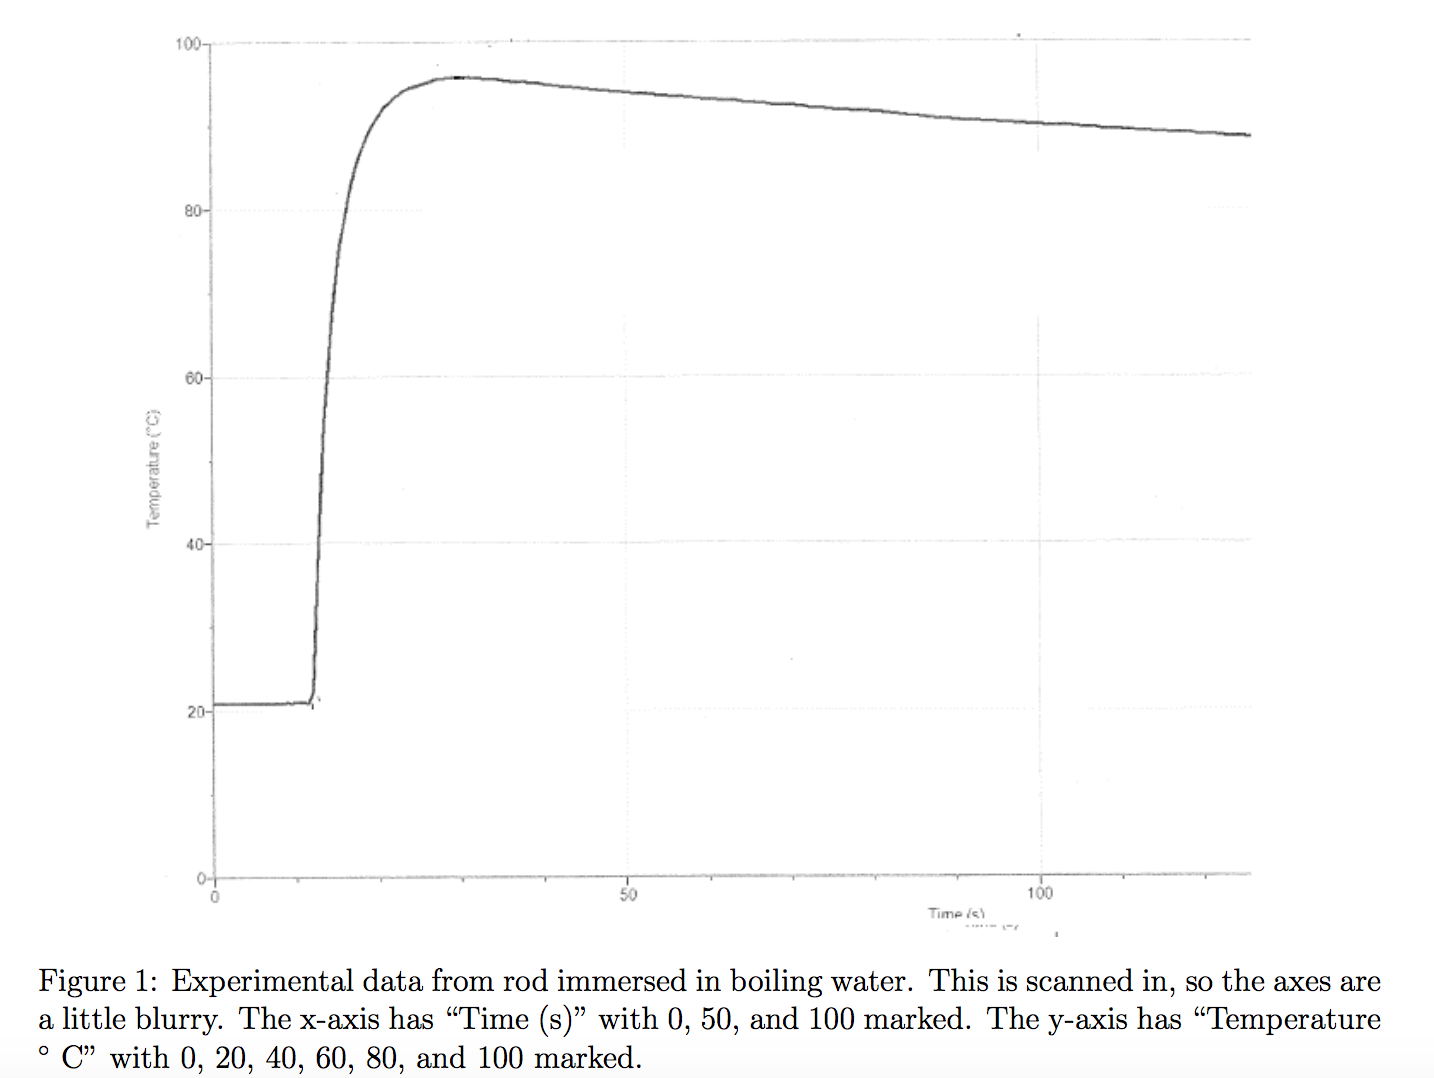
\includegraphics[width=13cm, height=8cm]{NewtonCool}

At $t=12s$, $T_r \approx 21^oC$

In our model, $T_r(0s) =21^oC$ was the initial condition, so that works out. Intuitively, this was the time that the rod was placed in the water, so there was no immediate temperature change- which makes sense, it takes time for the temperature of an object to change.

Looking at values of t between 12s and 22s, the graph shoots upwards, so let's plug some values into our model to check.

$T_r((13-12)s)=T_r(1s)= 38.7^oC$ (t=13s)

$T_r((17-12)s)=T_r(5s)= 75.9^oC$ (t=17s)

$T_r((21-12)s)= T_r(9s)=88.2^oC$ (t=21s)

This works out rather nicely, the values increase by a lot but it levels off as it goes to t=22s, so the increase from 17s to 21s should be a lot smaller than from 12s to 17s. It also seems like there is a maximum around t=30s to t=35s

$T_r((28-12)s)=T_r(16s)= 93.1^oC$ (t=28s)

$T_r((30-12)s)=T_r(18s)=93.3^oC$ (t=30s)

$T_r((32-12)s)=T_r(20s)= 93.4^oC$ (t=32s)

$T_r((34-12)s)=T_r(22s)= 93.3^oC$ (t=34s)

From our results, we definitely see that there is a peak around t=32s, and that the peak has a large width (moving a little from the peak doesn't change the value too drastically). Looking at the graph, this is exactly what we see. Furthermore, the values align quite well, simply eyeballing shows that the peak is at about $95^oC$. Now lets test for values after t=34s, from the graph, it should keep decreasing at a steady and slow rate.

$T_r((40-12)s)=T_r(28s)= 93.0^oC$ (t=40s)

$T_r((50-12)s)=T_r(38s)= 92.3^oC$ (t=50s)

$T_r((60-12)s)=T_r(48s)= 91.5^oC$ (t=60s)

$T_r((100-12)s)=T_r(88s)= 88.7^oC$ (t=100s)

$T_r((150-12)s)=T_r(138s)= 85.2^oC$ (t=150s)

From our results, it looks like it decreases at a steady amount, the slope is about $(-0.7/10)^oC/s = -0.07^oC/s$. from t=40s to t=60s, and the slope from t=100s to t=150s is about $(-3.5/50)^oC/s = -0.07^oC/s$, which matches the slope calculated earlier. Looking back at the graph, it does look linear from t=40s onwards, and the slope is quite small. Checking the values by eyeballing, at t=100s the temperature is about $90^oC$, which is very close to our value.









\end{document}
